\documentclass[
    % -- opções da classe memoir --
    12pt,               % tamanho da fonte
    openright,          % capítulos começam em pág ímpar (insere página vazia caso preciso)
    oneside,            % para impressão em verso e anverso. Oposto a oneside
    a4paper,            % tamanho do papel. 
    % -- opções da classe abntex2 --
    chapter=TITLE,      % títulos de capítulos convertidos em letras maiúsculas
    section=TITLE,      % títulos de seções convertidos em letras maiúsculas
    % -- opções do pacote babel --
    brazil              % o último idioma é o principal do documento
]{abntex2}

\usepackage{times}          % Usa a fonte Times
\usepackage[T1]{fontenc}    % Selecao de codigos de fonte.
\usepackage[utf8]{inputenc} % Codificacao do documento (conversão automática dos acentos)
\usepackage{lastpage}       % Usado pela Ficha catalográfica
\usepackage{indentfirst}    % Indenta o primeiro parágrafo de cada seção.
\usepackage{color}          % Controle das cores
\usepackage{microtype}      % para melhorias de justificação
\usepackage{listings}       % para inserir código fonte
\usepackage{graphicx}       % para inserir imagens

% Pacotes de citações
\usepackage[brazilian,hyperpageref]{backref}     % Paginas com as citações na bibl
\usepackage[alf]{abntex2cite}   % Citações padrão ABNT
\usepackage{titlesec}

% --- 
% CONFIGURAÇÕES DE PACOTES
% --- 

% altera o espacamento depois do número de cada secao, subsecao, etc
\titleformat{\section}
  {\normalfont\normalsize}{}{0pt}{\thesection\space}
\titleformat{\subsection}
  {\normalfont\normalsize\bfseries}{}{0pt}{\thesubsection\space}
\titleformat{\subsubsection}
  {\normalfont\normalsize}{}{0pt}{\thesubsubsection\space}
\titleformat{\paragraph}
  {\normalfont\normalsize\itshape}{}{0pt}{\theparagraph\space}

% ---
% Configurações do pacote backref
% Usado sem a opção hyperpageref de backref
\renewcommand{\backrefpagesname}{Citado na(s) página(s):~}
% Texto padrão antes do número das páginas
\renewcommand{\backref}{}
% Define os textos da citação
\renewcommand*{\backrefalt}[4]{
    \ifcase #1 %
        Nenhuma citação no texto.%
    \or
        Citado na página #2.%
    \else
        Citado #1 vezes nas páginas #2.%
    \fi}%
% ---

% ---
\titulo{\uppercase{Uma proposta de interface do cliente de torrent Transmission
                   baseado no GTK HIG 3.14}}
\autor{\uppercase{Derek Willian Stavis}}
\orientador{Aline Cristina Antoneli de Oliveira}
\orientadortcc{Prof. \imprimirorientador, Dr. (SENAI/SC)}
\coordenador{Prof. Luciana Schmitz, Esp. (SENAI/SC)}
\coordenadortcc{Profa. Jaqueline Voltolini de Almeida, Me. (SENAI/SC)}
\examinador{Prof. Fulado de tal, Me. (SENAI/SC)}
\preambulo{Trabalho de Conclusão de Curso apresentado à Banca Examinadora do
           Curso Superior de Tecnologia em Análise e Desenvolvimento de Sistemas
           da Faculdade de Tecnologia do SENAI Florianópolis como requisito 
           parcial para obtenção do Grau de Tecnólogo em Análise e 
           Desenvolvimento de Sistemas.}
\proforientador{Professor Orientador: \imprimirorientador.}
\datadefesa{\uppercase{28 de Novembro de 2014}}
\local{Florianópolis/SC}
\data{2014}

\instituicao{%
  SERVIÇO NACIONAL DE APRENDIZAGEM INDUSTRIAL 
  \par
  FACULDADE DE TECNOLOGIA SENAI/SC FLORIANÓPOLIS
  \par
  CURSO SUPERIOR DE TECNOLOGIA EM ANÁLISE E DESENVOLVIMENTO DE SISTEMAS}
\tipotrabalho{Trabalho de Conclusão de Curso}

% alterando o aspecto da cor azul
\definecolor{blue}{RGB}{41,5,195}

% informações do PDF
\makeatletter
\hypersetup{
        %pagebackref=true,
        pdftitle={\@title}, 
        pdfauthor={\@author},
        pdfsubject={\imprimirpreambulo},
        pdfcreator={LaTeX with abnTeX2},
        pdfkeywords={abnt}{latex}{abntex}{abntex2}{trabalho acadêmico}, 
        colorlinks=true,    % false: boxed links; true: colored links
        linkcolor=black,    % color of internal links
        citecolor=black,    % color of links to bibliography
        filecolor=magenta,  % color of file links
        urlcolor=black,
        bookmarksdepth=4
}
\makeatother
% --- 

% --- 
% Espaçamentos entre linhas e parágrafos 
% --- 

% O tamanho do parágrafo é dado por:
\setlength{\parindent}{1.3cm}

% Controle do espaçamento entre um parágrafo e outro:
\setlength{\parskip}{0.2cm}  % tente também \onelineskip

%\titlespacing\section{0pt}{12pt plus 4pt minus 2pt}{-6pt plus 2pt minus 2pt}

% ---
% compila o indice
% ---
\makeindex
% ---

% ----
% Início do documento
% ----
\begin{document}

% Retira espaço extra obsoleto entre as frases.
\frenchspacing 

% ----------------------------------------------------------
% ELEMENTOS PRÉ-TEXTUAIS
% ----------------------------------------------------------

\imprimircapa
\imprimirfolhaderosto*

\begin{folhadeaprovacao}

  \begin{center}
    {\ABNTEXchapterfont\bfseries\normalsize\imprimirautor}

    \vspace*{\fill}\vspace*{\fill}
    \begin{center}
      \ABNTEXchapterfont\bfseries\normalsize\imprimirtitulo
    \end{center}
    \vspace*{\fill}
        \imprimirpreambulo
    \vspace*{\fill}
        
   APROVADA PELA {\bfseries{COMISSÃO EXAMINADORA}}
   \par
   EM FLORIANÓPOLIS, \bfseries{\imprimirdatadefesa}
   \end{center}

   \assinatura{\imprimircoordenador \\ Coordenador do Curso} 
   \assinatura{\imprimircoordenadortcc \\ Coordenador de TCC} 
   \assinatura{\imprimirorientadortcc \\ Orientador} 
   \assinatura{\imprimirexaminador \\ Examinador}
   \begin{center}
    \vspace*{1cm}
  \end{center}
\end{folhadeaprovacao}

% Arquivos que devem ser alterados
% ====================================================================
% Dedicatória 
% ====================================================================
\begin{dedicatoria}

\end{dedicatoria}

% ====================================================================
% Agradecimentos 
% ====================================================================
\begin{agradecimentos}
Em primeiro lugar, agradeço a meus pais. Sem eles eu não estaria aqui.

Em segundo, agradeço a internet, cada site e cada pessoa que pôde me fazer
entender e conhecer algo que eu não sabia.
\end{agradecimentos}

\begin{epigrafe}
    \vspace*{\fill}
	\begin{flushright}
		\textit{``A única coisa que não muda é que tudo muda.''} \\
		(HERÁCLITO DE ÉFESO)
	\end{flushright}
\end{epigrafe}


\noindent STAVIS, Derek Willian. \textbf{\imprimirtitulo} Florianópolis, 2015.
\pageref{nropaginas}f. Trabalho de Conclusão de Curso Superior de Tecnologia em
Análise e Desenvolvimento de Sistemas. Faculdade de Tecnologia do SENAI,
Florianópolis, 2015.

\vspace{1cm}
\setlength{\absparsep}{18pt} % ajusta o espaçamento dos parágrafos do resumo
\begin{resumo}

  Os avanços trazidos nos últimos quatro anos no ambiente gráfico GNOME foram de
  suma importância para atingir uma experiência diferenciada e consistente de
  uso. Conceitos já difundidos no design de interfaces de usuário foram
  revisitados, paradigmas foram quebrados, mudando a forma com que os usuários
  vêem e interagem com o sistema operacional. Entretanto, nem todos os softwares
  disponíveis para a plataforma acompanharam a velocidade de desenvolvimento da
  plataforma GNOME, e muitos ainda necessitam de atenção. Com o lançamento do
  HIG (Guia de Interface com o Usuário) no GNOME versão 3.12 toda filosofia e
  padrões de design da plataforma foram sintetizados em linguagem simples e
  objetiva, tornando-se o material referência para o desenvolvimento e
  manutenção de seu ecosistema de softwares. Esta pesquisa aborda o processo de
  adaptação do cliente de torrent Transmission de acordo com o guia de
  interfaces do GNOME versão 3.14.

  \vspace{\onelineskip}

  \noindent
  \textbf{Palavras-chave}: Interfaces Gráficas. GTK+. GNOME. Design. Redesign.

\end{resumo}

% ====================================================================
% Abstract 
% ====================================================================
\noindent
STAVIS, Derek Willian. \textbf{Uma proposta de interface do cliente de torrent Transmission baseado no GTK HIG 3.14}
Florianópolis, 2013. 89f. Trabalho de Conclusão de Curso Superior de Tecnologia 
em Análise e Desenvolvimento de Sistemas. Faculdade de Tecnologia do SENAI,
Florianópolis, 2013.

\vspace{1cm}
\begin{resumo}[\textbf{ABSTRACT}]
 \begin{otherlanguage*}{english}
   This is the english abstract.

   \vspace{\onelineskip}
 
   \noindent 
   \textbf{Key-words}: Graphical User Interfaces. GTK+. GNOME. Design. Redesign.
 \end{otherlanguage*}
\end{resumo}



% lista de figuras
\pdfbookmark[0]{\listfigurename}{lof}
\listoffigures*
\clearpage

% inserir lista de tabelas
\pdfbookmark[0]{\listtablename}{lot}
\listoftables*
\clearpage

% Arquivos que devem ser alterados
% ====================================================================
% Siglas 
% ====================================================================

\begin{siglas}
  \item[GTK] GIMP Toolkit - Biblioteca de componentes para criação de interfaces gráficas.
  \item[GIMP] GNU Image Manipulation tool - Ferramenta de manipulações de imagem de código aberto, sob licensa GNU.
  \item[GNOME] Ambiente gráfico de estação de trabalho disponível para GNU/Linux.
  \item[GNU/Linux] Distribuição de software de código aberto que forma a base de um sistema operacional.
\end{siglas}


\include{content/simbolos}

% inserir o sumario
\pdfbookmark[0]{\contentsname}{toc}
\tableofcontents*
\clearpage

% ----------------------------------------------------------
% ELEMENTOS TEXTUAIS
% ----------------------------------------------------------
\textual

% PARTE - preparação da pesquisa
% ----------------------------------------------------------
%\part{Preparação da pesquisa}


% Informações que devem ser alteradas
% **************************************************
% ---
% Introdução
% ---
\chapter{INTRODUÇÃO}

O lançamento de um guia de padrões para o desenvolvimento de interfaces gráficas
orientadas ao ambiente gráfico GNOME foi de suma importância para alinhar
desenvolvedores ao intuito deste ambiente gráfico de código aberto.

O guia contribui para que o GNOME passe a ter mais harmonia visual, seja através
dos aplicativos centrais, -- os primeiros a receber tratamento estético -- ou
por aplicativos de terceiros, que devem se adaptar utilizando o guia como
referência.

Aplicativos que não se adequam ao guia passam a apresentar-se defasados,
perdendo pontos em usabilidade e em beleza, e aumentando a taxa de rejeição.
Mantenedores de aplicativos baseados no toolkit GTK devem, portanto, dedicar
atenção para o fator de usabilidade e o progresso da plataforma quais foram
desenhados para.

Um aplicativo que sofre deste efeito e necessita dedicação é o Transmission, um
cliente de torrent popular, que foi desenvolvido na era GTK 2, onde os
requisitos, recursos e a visão da plataforma GNOME eram diferentes
\cite{gnome221hig}.

O objetivo principal desta pesquisa é explorar o HIG do GTK 3.14, além de
avançar o desenvolvimento de um software livre mantido pela comunidade de código
aberto, propondo e contribuindo melhorias visuais e de código-fonte na interface
gráfica do Transmission.

Esta pesquisa foi baseada na análise de diversos casos de uso de softwares
contidos na plataforma GNOME Desktop, versão 3.14, e tem a pretensão de
descrever o processo de pensamento e a motivação por trás das adaptações de
interface gráficas propostas.

\section{OBJETIVOS}

\subsection{Objetivo geral}

Propor adaptações na interface gráfica GTK do cliente de torrent Transmission de
acordo com as recomendações do HIG versão 3.14, trazendo mais harmonia para seus
utilizadores na plataforma GNOME.

\subsection{Objetivos específicos}

\begin{enumerate}
  \item Comparar dados evolutivos da interface de aplicações centrais do GNOME.
  \item Identificar pontos de redesign na janela principal do Transmission.
  \item Propor adaptações na interface do Transmission, embasadas no HIG 3.14.
\end{enumerate}

O desenvolvimento de mecanismos que automatizam tarefas existe desde a idade das
pedras, onde hominídeos produziam ferramentas para auxílio próprio. A
transversalidade do conhecimento e da experimentação nos levou a descoberta de
novas metodologias e o aperfeiçoamento de técnicas, consequentemente modificando
a forma com que o ser humano interage com o mundo \cite[p.
1]{sartori2010neurociencia}.

\section{Interfaces gráficas}

O conceito de interface é extremamente amplo, e foi largamente difundido com o
início dos estudos de interação humano-máquina. O avanço da industrialização
permitiu com que máquinas extremamente complexas substituíssem seres humanos nas
tarefas mais difíceis,  deixando estes, seus operadores, apenas com a
responsabilidade de pilotá-las de forma simples e segura.

O advento de tecnologias multimídias interativas como computadores, celulares e
tablets elevou o patamar da criação de interfaces e gestão de tarefas ao estado
da arte, agregando conhecimentos transversais de artistas visuais a músicos.

\citeonline[p. 1]{ferreira2005semiotics} afirmam que a criação de “interfaces
com o usuário ainda está mais para arte do que para ciência.", e justificam,
explicando que "A maior parte do design ou redesign é baseado em estudos
empíricos ou protótipos, e ainda há muito pouca compreensão teórica ou de
engenharia de como conduzir o processo de design e produzir bons designs pela
primeira vez”.

O primeiro conceito científico de gerenciamento de tarefas através da
sobreposição de janelas data de 1969, na tese de Ph.D. de Alan Kay. A
implementação de seu conceito, vista pela primeira vez em funcionamento no
sistema do Xerox PARC, é largamente utilizada até hoje por grandes sistemas
tanto comerciais quanto de código aberto, como Windows, OS X, GNOME, KDE
\cite[p. 7]{myers2000past}.

Interfaces gráficas modernas foram alcançadas através da associação entre
hardware e software, utilizando de diversos dispositivos de entrada e saída,
além de  inúmeras camadas de software, com o intuito de promover usabilidade e
fácil adaptação.

Dispositivos de entrada transformam coordenadas do mundo real para o mundo
virtual, registrando condições externas que podem ser modificadas através da
interação com um ou mais atores. Dispositivos de entrada comuns são mouse, tela
de toque, teclado, etc.

Dispositivos de saída projetam informações geradas por um sistema computacional
e seu caráter é geralmente baseado nos sentidos: Visão, audição, tato. O
dispositivo de saída mais comum é o monitor, que tem por finalidade projetar
imagens compatíveis com a capacidade humana de visão.

\section{Gerenciadores de Janelas e Toolkits}

Gerenciadores de janelas suportam a separação da imagem de um dispositivo de
saída (geralmente monitores) em múltiplas regiões de desenho, comumente chamadas
de janelas  \cite[p. 5]{myers1996uimss}.

Um gerenciador de janelas moderno também tem por finalidade coordenar a exibição
de um conjunto de janelas em um conjunto de monitores, escutar por eventos de
entrada (mouse, teclado) e informar os responsáveis pelas janelas sobre
alterações no layout de tela (dimensões da tela, dimensões da janela, espaço de
cor).

Gerenciadores de janelas, porém, não tem por responsabilidade preencher as áreas
de desenho com gráficos, e como suas APIs operam geralmente a nível de pixel, a
tarefa de escrever um programa gráfico acaba sendo demorada e entediante.
\apudonline{rosenthal1988simple}{myers2000past}. Além disso, se cada
desenvolvedor criasse seus próprios componentes, seria praticamente impossível
disponibilizar uma experiência consistente ao usuário.

Para solucionar este problema ferramentas conhecidas como toolkits foram criadas
sobre as abstrações disponibilizadas pelos WMs. Sua finalidade é esconder
características de baixo nível, disponibilizando uma fachada homogênea e
portável para o desenvolvedor de software, além de comportamento e experiência
visual consistente para o usuário final \cite{myers2000past}.

As responsabilidades de um toolkit incluem desenhar elementos de interface
gráfica como texto, botões, imagens, barras de progresso, etc, de acordo com um
ou mais estilos visuais. Também é sua responsabilidade processar eventos de um
ou mais dispositivos de entrada (mouse, teclado, painel de toque) verificar a
colisão de um evento com elementos de interface gráfica (clique em um botão, por
exemplo), traduzir e informar os eventos para a aplicação proprietária da
janela.

Toolkits multiplataforma podem ser utilizados para escrever interfaces gráficas
portáveis, permitindo com que o mesmo código seja recompilado para um sistema
operacional diferente do em que foi escrito e funcione da mesma forma.

\section{A plataforma GNOME e o toolkit GTK}

Existem diversas opções de gerenciadores de janela de código aberto, comumente
incluídos em várias distribuições de Linux. O GNOME, um ambiente gráfico
bastante difundido pelos usuários de Linux, foi fundado e está em constante
desenvolvimento por uma comunidade de engenheiros de software ao redor do mundo.

Muito além de um mero gerenciador de janelas, a plataforma GNOME se desenvolveu
a ponto de ser constituída por uma série de aplicações base, incluindo um
gerenciador de janelas, um lançador de aplicações e diversos aplicativos
integrados, como calculadora, editor de texto, gerenciadores de arquivos, redes,
contatos, etc.

A plataforma GNOME e seus aplicativos integrados são altamente baseados no
toolkit GTK. De acordo com o site oficial, o ”GTK +, ou GIMP Toolkit, é um
conjunto de ferramentas multi-plataforma para criar interfaces gráficas de
usuário. Oferecendo um conjunto completo de widgets, o GTK + é adequado para
projetos desde pequenas ferramentas pontuais até suítes completas de
aplicativos.”  [1].

\section{O código aberto e desenvolvimento contínuo}

Uma das característica das plataformas de código aberto é a distribuição de
esforços em prol do constante desenvolvimento e melhoria. A pluralidade de
opiniões e idéias eleva o patamar das discussões e permite com que vários pontos
de vista sejam levados em consideração na evolução da plataforma.

Apesar dos prós existentes na distribuição de esforços também existem os contras
— Projetos que são desenvolvidos paralelamente nem sempre avançam na mesma
velocidade. E o contra fica mais sério quando um projeto depende do outro, como
é o caso de toolkits e programas que consomem suas APIs (Application Programming
Interfaces - Interfaces Programador-Programa).

Além dos aplicativos integrados, geralmente garantidos de acompanhar a evolução
da plataforma, sua ergonomia e visual, existe uma vasta gama de aplicações tanto
de código aberto quanto proprietárias disponíveis para atender as mais variadas
necessidades. Em sua grande maioria os aplicativos também são mantidos pela
comunidade, e se não atualizados podem ficar defasados em usabilidade, ergonomia
e consistência com a plataforma.

\section{Impactos na consistência e usabilidade}

Shneiderman, 1992 descreve a usabilidade como uma combinação das seguintes
características:

\begin{itemize}
    \item Facilidade de aprendizado
    \item Alta velocidade de operação
    \item Baixa taxa de erros
    \item Satisfação do usuário
    \itemRetenção de usuários pelo tempo
\end{itemize}

Em prol da usabilidade a maioria dos toolkits aplica um modelo próprio de
apresentação, organização, interação e estilização de widgets, que
costumeiramente varia de acordo com o tipo de ambiente onde é executado
(desktop, tablet e celular).

O conjunto de padrões de design recomendado ao utilizar o GTK para garantir a
máxima usabilidade da plataforma foi especificado oficialmente através de um
documento lançado no ano de 2014, acompanhando a versão 3.14 do toolkit, sob o
título de Human Interface Guidelines.

O HIG, como também é chamado, é uma literatura ilustrada de diretrizes
recomendadas no desenvolvimento de interfaces gráficas que utilizem o toolkit,
com o intuito de reforçar a consistência visual e integração com diferentes
gerenciadores de janela.

\section{Estudo de caso: Transmission}

Um aplicativo famoso disponível para a plataforma GNOME é o cliente de
BitTorrent Transmission. Aclamado pela sua simplicidade, o aplicativo é
utilizado para compartilhar arquivos através da internet.

A interface gráfica do Transmission foi desenvolvida na era GNOME 2, e por mais
que componentes básicos como botões e listas não tenham mudado agressivamente no
GNOME 3, muitos padrões de design foram criados ou mudaram, trazendo mais
conforto e consistência para os usuários e desenvolvedores do toolkit.

O objetivo principal desta pesquisa é explorar o HIG do GTK 3.14, além de
avançar o desenvolvimento de um software livre mantido pela comunidade de código
aberto, propondo e contribuindo melhorias visuais e de código-fonte na interface
gráfica do Transmission.

Esta pesquisa foi baseada na análise de diversos casos de uso de softwares
contidos na plataforma GNOME Desktop, versão 3.14, e tem a pretensão de
descrever o processo de pensamento e a motivação por trás das adaptações de
interface gráficas propostas.


\chapter{PROCEDIMENTOS METODOLÓGICOS}

A presente pesquisa aplicada foi desenvolvida através da exploração de casos de
uso tanto da evolução de aplicativos centrais da plataforma GNOME quanto padrões
de design utilizados em outras versões do cliente de torrent Transmission.

Segundo \citeonline{jung2003metodologia}, o objetivo da pesquisa aplicada é
gerar inovação frente a uma demanda ou necessidade, e seu desenvolvimento
consiste na utilização dos conhecimentos adquiridos na pesquisa básica
associados a pesquisa tecnológica, com a finalidade de obter aplicações
práticas.

O produto final desta pesquisa se concretiza na forma de um protótipo funcional
de interface gráfica compatível com os padrões definidos no HIG 3.14 para o
cliente de torrent Transmission.

\section{Estudo longitudinal dos padrões de design nas aplicações}
\label{sec:chronologic-analysis}

Através de pesquisa exploratória com o objetivo de avaliar o processo de
evolução da plataforma GNOME e seu design, foram identificadas aplicações
centrais do GNOME 3.16 que já implementam os padrões de design definidos pelo
HIG \cite{gnome314hig}.

\citeonline{jung2003metodologia} caracteriza a pesquisa exploratória pela
extração de conhecimento sobre um dado fenômeno, sem grande teorização, visando
descobrir práticas e diretrizes alternativas ao conhecimento existente.

Foram escolhidas três aplicações centrais a serem analisadas. Pelo papel
significativo desempenhado na experiência GNOME foram selecionadas as seguintes
aplicações:

\begin{itemize}
    \item Nautilus -- Navegador de Arquivos
    \item Evince -- Visualizador de Documentos Digitais
    \item Gedit -- Editor de Arquivos de Texto
\end{itemize}

Com propósito de avaliar a dinâmica do processo de design do GNOME ao longo do
tempo, um estudo de caráter longitudinal foi elaborado nas três aplicações
escolhidas, através da comparação de duas versões distantes do GNOME e das
aplicações centrais escolhidas.

A montagem do ambiente necessário para a execução do estudo longitudinal foi
facilitada pela distribuição oficial de sistemas operacionais com todo software
necessário para uma experiência GNOME básica, prontos para usar através da
transferência para uma mídia inicializável \cite{gnome2015promo-usb}. Detalhadas
na \autoref{gnome-versions} estão as informações das versões escolhidas, dentre
as disponíveis para estudo.

A soma de verificação de cada arquivo foi utilizada para checar a integridade do
sistema operacional, e todas aplicações foram analisadas na versão oficial --
sem alterações na configuração do sistema, troca de temas, fontes, etc.

\begin{table}[htb]
\ibgetab{
  \caption{Sistemas operacionais e versões do GNOME}
  \label{gnome-versions}
}{
  \begin{tabularx}{\textwidth}{ | l | l | l | X | }
  \hline
  Versão do GNOME & Data de Modificação & Nome do arquivo & Soma de Verificação \\
  \hline
  3.6.0 & 08/10/2012 & GNOME-3.6.0.iso       & MD5:
                                               753c99ce2342f658
                                               65c1f74bc3722e44 \\
  \hline
  3.16  & 25/03/2015 & gnome-3.16.x86-64.iso & SHA256:
                                               4a6185a0aca89f15
                                               8f769d76d5a0086f
                                               0f1e9d709a5d80cd
                                               cf2b0d52d67ab2b2 \\
  \hline
  \end{tabularx}
}{
  \fonte{\cite{gnome2015promo-usb}}
}
\end{table}

Dentre os diversos padrões de design especificados pelo HIG
\cite{hig314patterns} foram selecionados cinco padrões de interesse a serem
analisados no estudo:

\begin{enumerate}
  \item Menu da Aplicação
  \item Janela Primária
  \item Barra de Título
  \item Comutador de Visão
  \item Busca
\end{enumerate}

As variáveis observadas no estudo incluiram, porém não se limitaram a (i) área
útil vs controles, onde foi analisada a razão entre a quantidade de pixels de
área útil versus controles da aplicação e (ii) relocação de funcionalidade,
onde foram analisadas mudanças operacionais em um mais elementos de interface,
sendo estas de caráter quantitativo e qualitativo, respectivamente.

A obtenção da razão área útil versus controles foi feita através da medição em
pixels da janela principal de cada aplicativo Foi considerada área útil a área
do aplicativo na qual a informação principal é apresentada, conforme
exemplificado na \autoref{workarea-chrome-ratio}. No caso do Nautilus, a lista
de arquivos é a área principal, do Evince, o documento apresentado, e no caso do
Gedit, a área de edição de texto.

\begin{figure}[h!]
  \begin{center}
    \caption{\textbf{Medição da razão área útil vs controles}}
    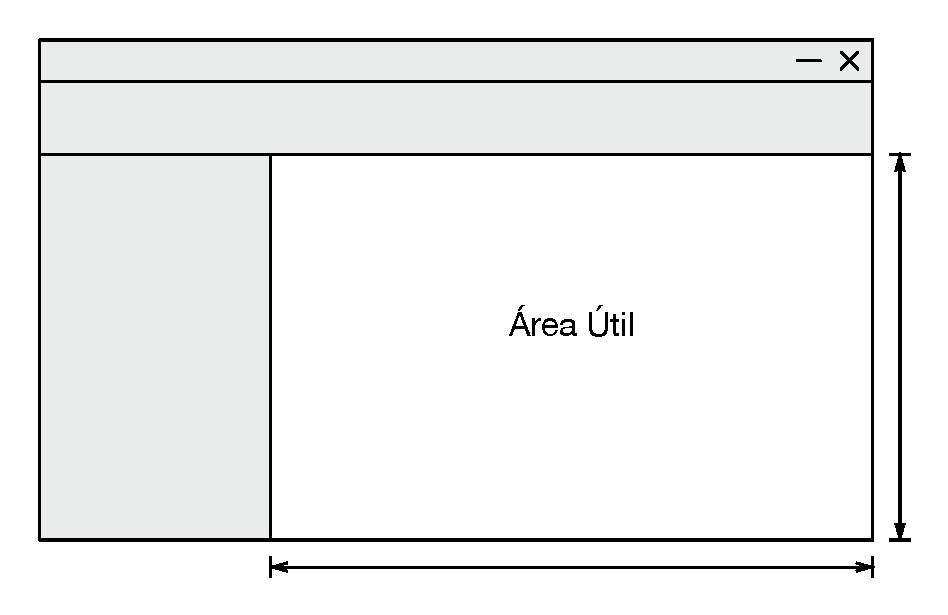
\includegraphics[scale=0.7]{image/workarea-chrome-ratio.eps}
    \fonte{Do Autor}
    \label{workarea-chrome-ratio}
  \end{center}
\end{figure}

A relocação de funcionalidades analisou a transição de um elemento de interface,
onde um menu, por exemplo, pode ter sido transformado em um botão, movido para
outro local, etc.

\section{Proposição de melhorias na interface do Transmission}

\citeonline{de2009client} afirmam que a prototipação de interfaces é uma técnica
de evolução de design que tem como base a constante interação e avaliação dos
resultados. \citeonline[p. 2]{baumer1996user} classifica e separa em quatro
classes os protótipos de interfaces gráficas:

\begin{enumerate}
  \item De apresentação
  \item Funcional
  \item Experimental
  \item Piloto
\end{enumerate}

Pela (i) maleabilidade de implementar estrategicamente ambas interface gráfica e
funcionalidade de um programa, com o propósito de averiguar o funcionamento de
um conceito e (ii) pelo fato do Transmission permitir alterações em seu código-
fonte através de sua licença GPL o protótipo funcional foi escolhido como método
experimental para a geração de propostas de melhorias na interface do
Transmission.

O protótipo funcional foi gerado através de alterações experimentais no código-
fonte do Transmission objetivando modificar sua interface gráfica utilizando
como base as tendências encontradas no estudo logitudinal das aplicações
centrais e também as diretivas estabelecidas no HIG.


\chapter{RESULTADOS E DISCUSSÕES}

A \autoref{transmission-prototype} apresenta o protótipo funcional
resultado da aplicação desta pesquisa, embasado na análise das aplicações
centrais e estudo do HIG, gerado através da alteração do código-fonte do
\textit{Transmission} versão 2.82.

\begin{figure}[!ht]
  \begin{center}
    \caption{\textbf{Protótipo funcional do \textit{Transmission} no GNOME 3.16}}
    \includegraphics[width=\textwidth]{image/transmission-gtk3-main.png}
    \label{transmission-prototype}
    \fonte{Do Autor (2015)}
  \end{center}
\end{figure}

Verificou-se que o embasamento nos dados evolutivos das aplicações centrais do
GNOME foi de grande utilidade para compreender o processo de redesign dos
aplicativos desta plataforma, possibilitando e facilitando a geração das
propostas de redesign do \textit{Transmission}.

\section{Percepções do processo de transição das aplicações centrais}

Durante o processo de análise longitudinal percebeu-se uma tendencia clara de
redução da razão área útil vs controles em todas aplicações centrais analisadas.
Também foi possível perceber a padronização da razão na versão 3.16 de todas as
aplicações. A \autoref{workarea-vs-chrome} apresenta as razões área útil vs
controles calculadas, enquanto a figura \autoref{coreapps-workarea-vs-chrome}
ilustra o processo de aquisição.

\begin{table}[htb]
\ibgetab{
  \caption{Área útil vs Controles}
  \label{workarea-vs-chrome}
}{
    \begin{tabular}{ | l | l | l | } 
    \hline
    Aplicação & Versão 3.6 & Versão 3.16 \\
    \hline
    \textit{Nautilus}  & 0.17       & 0.07 \\
    \textit{Evince}    & 0.18       & 0.07 \\
    \textit{Gedit}     & 0.16       & 0.07 \\
    \hline
    \end{tabular}
}{
  \fonte{Do Autor (2015)}
}
\end{table}

\begin{figure}[!ht]
  \begin{center}
    \caption{\textbf{Aquisição das razões área útil vs controles}}
    \includegraphics [width=\textwidth]{image/coreapps-workarea-chrome-ratio.eps}
    \label{coreapps-workarea-vs-chrome}
    \fonte{Do Autor (2015)}
  \end{center}
\end{figure}


A tendência de redução desta razão se repete na remodelagem da forma e função de
vários widgets, uma clara influência de ambos design de usabilidade e da redução
de espaço vertical, visto a padronização de resoluções baseados na razão 16:9
(720p, 1080p, etc).

Falando especificamente sobre os elementos de interface, um dos elementos mais
comuns de um ambiente gráfico baseado em janelas é a barra de título, por onde o
usuário pode mover a janela no espaço de trabalho. Até então, no GNOME,
desenvolvedores tinham pouco ou nenhum controle sobre elas por questões de
compatibilidade de software.

Com a introdução do conceito de \textit{Header Bar}, as antigas barras de título
passam a acomodar botões, caixas de texto, sliders, etc, substituindo as barras
de ferramentas, antes encontradas comumente abaixo de menus ou das barras de
título, conforme a \autoref{toolbar-positioning}.

\begin{figure}[!ht]
  \begin{center}
    \caption{\textbf{Barra de Ferramentas no \textit{Evince} e \textit{Gedit} 3.6}}
    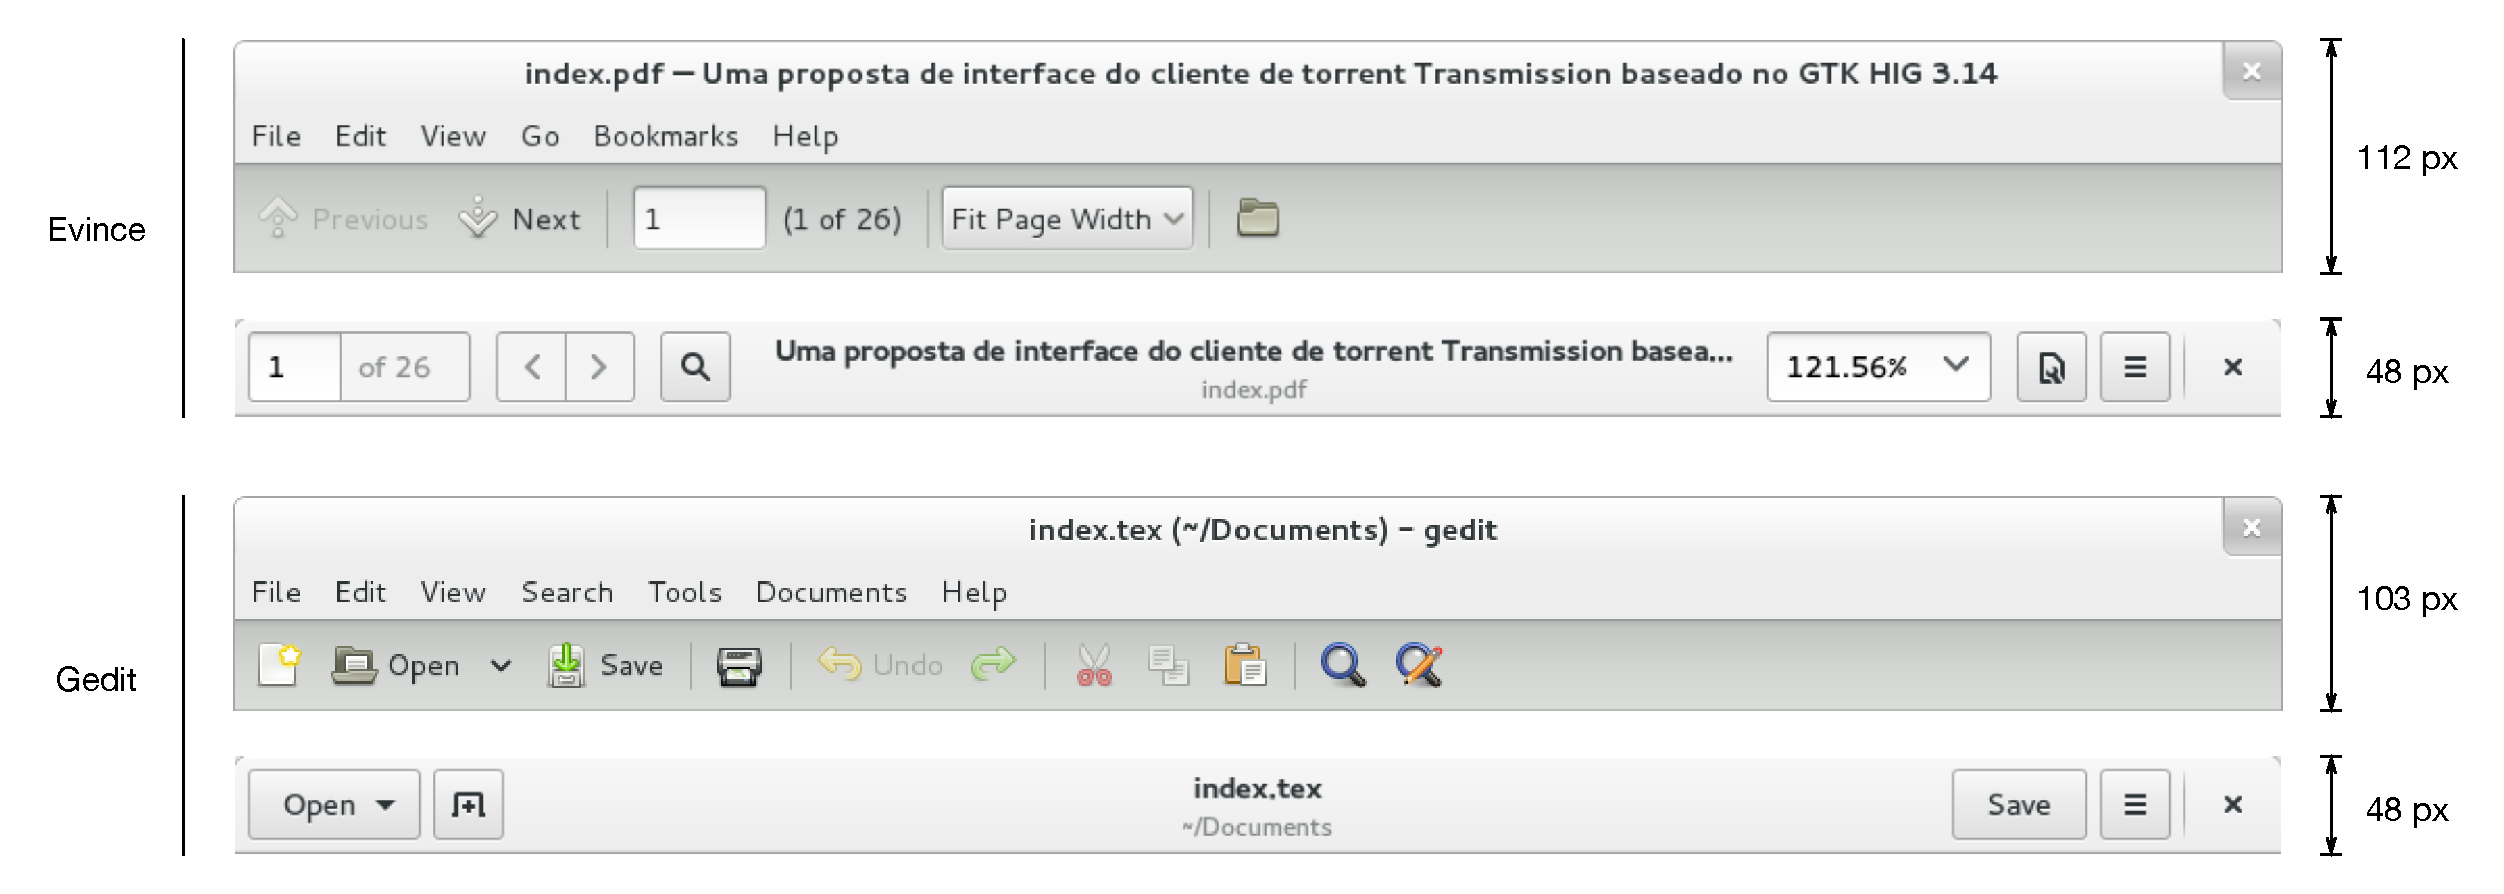
\includegraphics [width=\textwidth]{image/toolbar-headerbar-comparison.eps}
    \fonte{Do Autor (2015)}
    \label{toolbar-positioning}
  \end{center}
\end{figure}

Constatou-se que, dentre as aplicações analisadas na versão 3.6, o
\textit{Nautilus} foi a mais avançada em relação aos padrões de design definidos
pelo HIG, antes mesmo deste guia ser publicado, através da pré-implementação de
uma \textit{Header Bar}, abaixo da barra de título, evidenciando a
experimentação progressiva dos novos padrões antes de uma aplicação geral.

Outra mudança notável foi a transição da barra de menus, quais ações foram
dissolvidas através de um ou mais widgets na janela do programa (sendo grande
maioria na \textit{Header Bar}), nas ações pertinentes a janela, e em um menu de
aplicação, para ações pertinentes ao programa (Abrir, Sobre, Sair). A
\autoref{rip-menubar} apresenta um mapeamento aproximado das ações da barra de 
menus do \textit{Evince} 3.6 para o 3.16.

\begin{figure}[!ht]
  \begin{center}
    \caption{\textbf{Mapeamento de menu no \textit{Evince}}}
    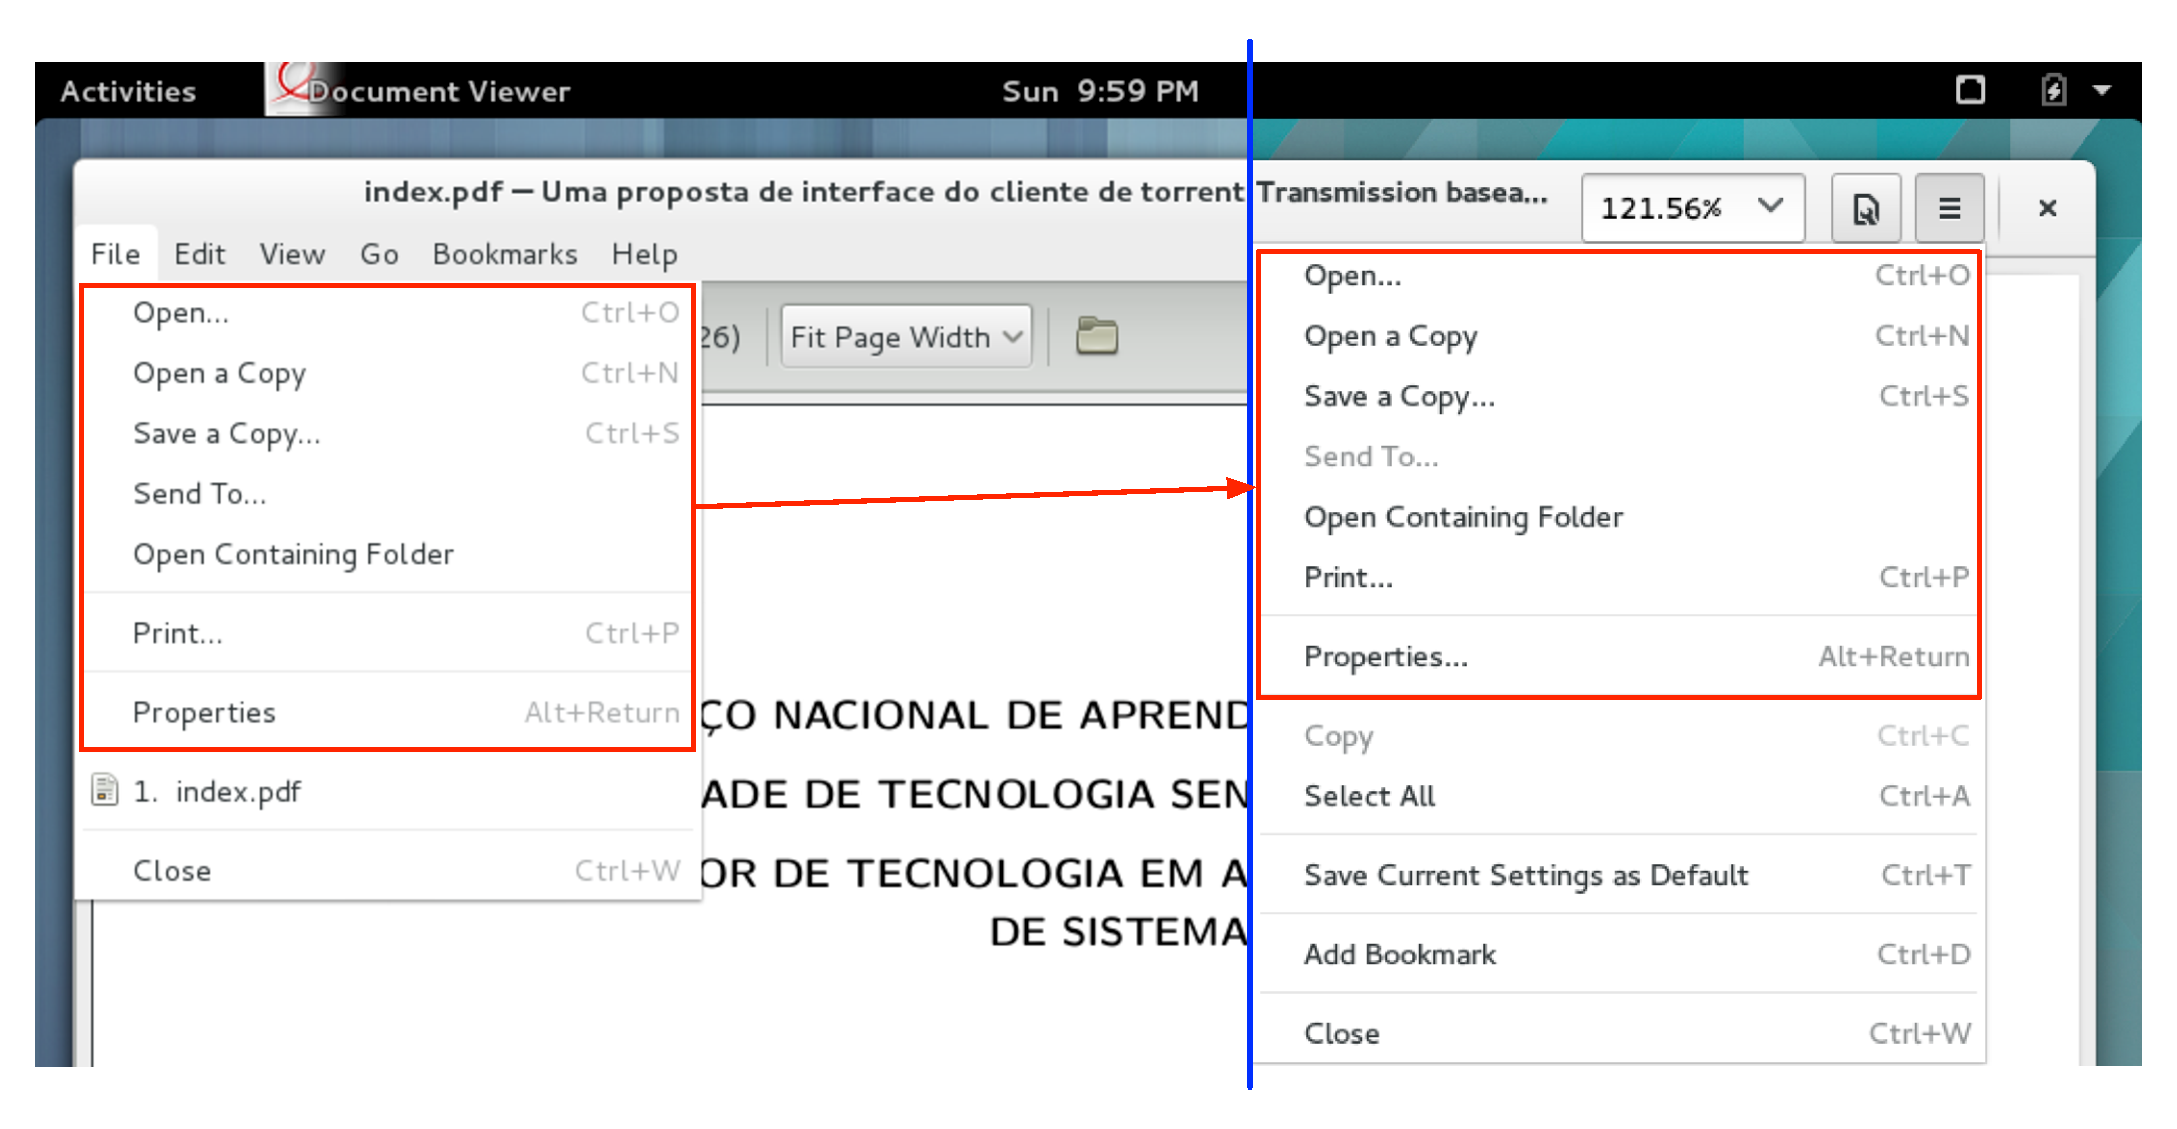
\includegraphics [width=\textwidth]{image/evince-menubar-mapping.eps}
    \fonte{Do Autor (2015)}
    \label{rip-menubar}
  \end{center}
\end{figure}

A utilização do \textit{Revealer} em ambos \textit{Nautilus} e \textit{Evince}
também demonstrou-se eficaz como técnica para redução de espaço vertical e
aumento da área útil de ambos programas, através da exibição temporária da caixa
de busca, alternável pelo botão lupa no \textit{Header Bar}.

O \textit{Popover}, um elemento de interface introduzido no HIG 3.12, é uma
visão alternável e flutuante que permitite adicionar menus, listas e widgets
variados em seu interior, e é comumente usado como parte de menus ou menus de
contexto. Sua utilização foi observada em diversos pontos, inclusive como
coadjuvante na transição da barra de menus em todas aplicações analisadas.

\section{Processo de redesign da interface do textit{Transmission}}

Em relação a utilização do \textit{Transmission} após o contato com as
aplicações centrais do GNOME 3.16 fica claro, logo na primeira utilização, que
sua interface não adere aos padrões incluídos no HIG, e se mostra completamente
desatualizada.

Foi possível, através da análise da transição das aplicações centrais do GNOME,
compilar uma série de modificações que podem ser aplicadas em prol da melhoria
da compatibilidade da interface do \textit{Transmission} com a experiência
GNOME, quais serão apresentadas a seguir.

\subsection{Header Bar}

A implementação da \textit{Header Bar} no \textit{Transmission} foi efetivada
através da dissolução das ações encontradas em ambas barra de ferramentas e
menus em botões. As ações da barra de menus foram separadas em duas categorias
de menu: Ações pertinentes ao programa e ações pertinentes a transferência
selecionada, posicionados da direita para a esquerda, respectivamente, conforme
indicado pelo HIG.

A \autoref{header-bar-transition} apresenta um paralelo entre a interface antiga
e a interface proposta, relacionando através de marcação em cores as transições
efetuadas. Os botões sensíveis a selecão (Iniciar, Parar e Remover) puderam ser
mantidos com seu comportamento original.

\begin{figure}[!ht]
  \begin{center}
    \caption{\textbf{Transição da \textit{Header Bar}}}
    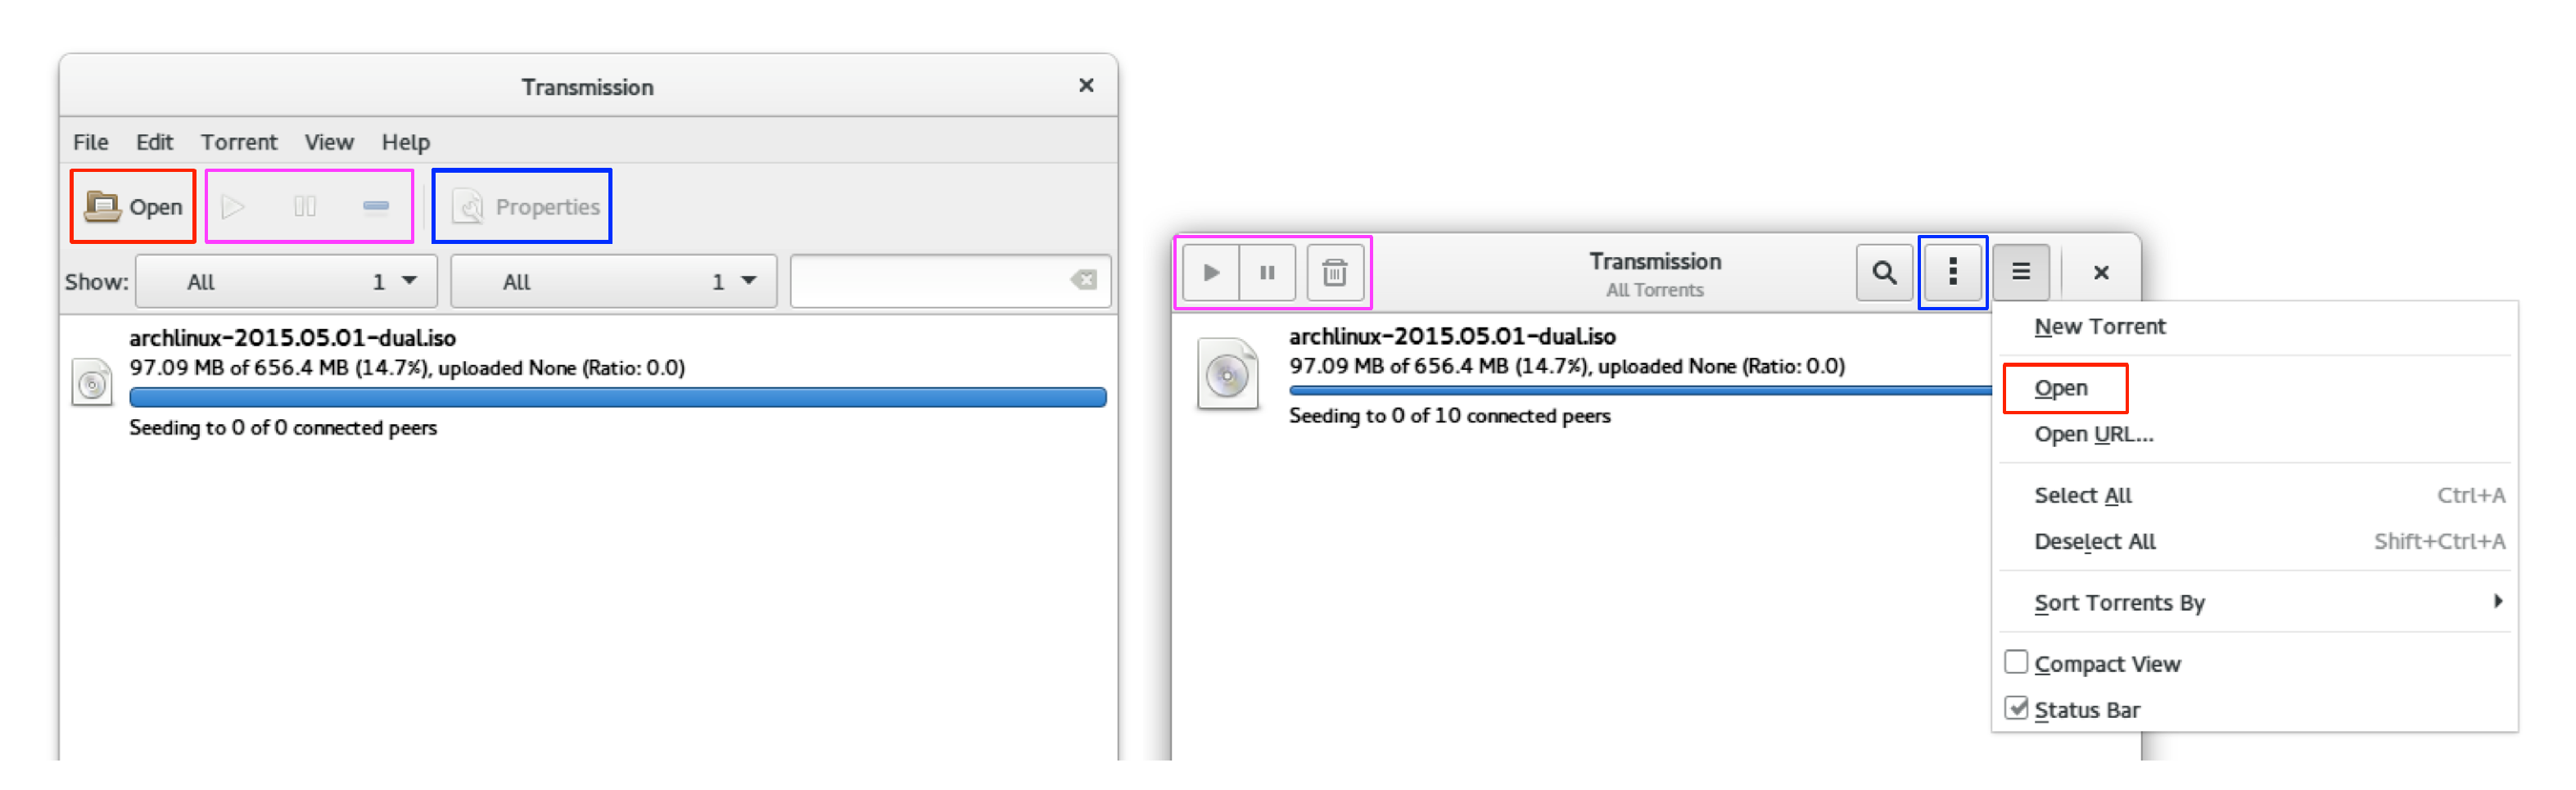
\includegraphics [width=\textwidth]{image/header-bar-transition.eps}
    \label{header-bar-transition}
    \fonte{Do Autor (2015)}
  \end{center}
\end{figure}

Pela natureza compacta da janela do \textit{Transmission} e pelo
compartilhamento do espaço disponível na \textit{Header Bar} pelos botões de
ação e título da aplicação, a adição excessiva de botões pode suprimir o título
da janela, e a presença de um número diferente de botões no lados direito e
esquerdo pode fazer parecer com que o título não esteja centralizado, causando
desconforto visual. Por este motivo os botões ``Properties'' e ``Open'' foram
migrados para os menus, sendo este movido para o menu de janela e aquele para o
menu de seleção.

\subsection{Barra de Filtros}

Seguindo a implementação utilizada no \textit{Evince} e \textit{Nautilus}, os
filtros de atividade foram movidos juntamente a caixa de busca textual para um
\textit{Revealer}, ativado através do botão com ícone de lupa, destacado na
\autoref{revealer}.

\begin{figure}[!ht]
  \begin{center}
    \caption{\textbf{Filtros retráteis através do uso de um Revealer}}
    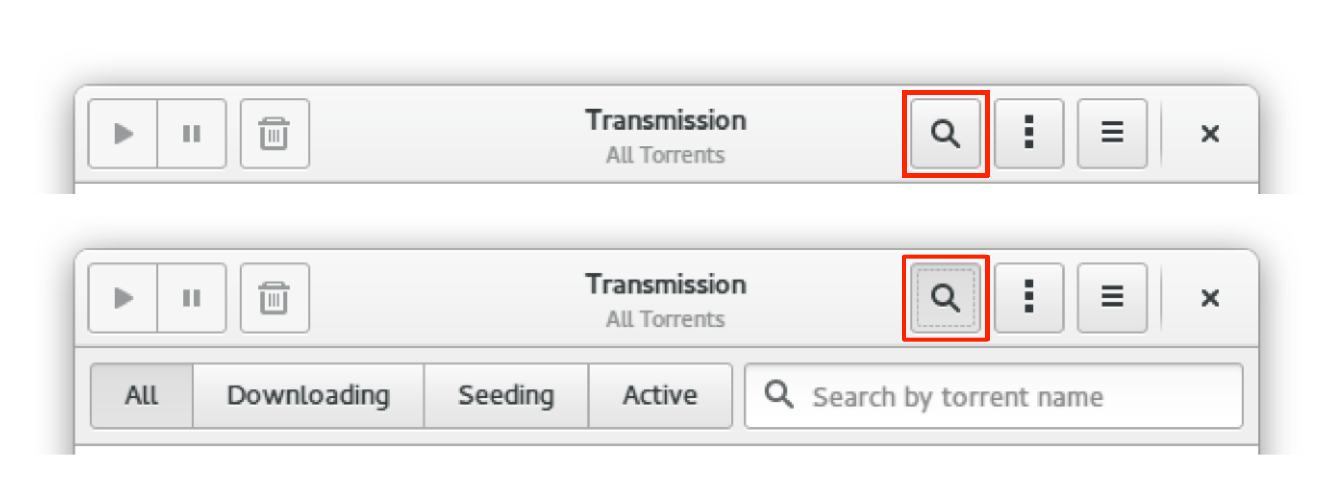
\includegraphics [width=\textwidth]{image/revealer.eps}
    \label{revealer}
    \fonte{Do Autor (2015)}
  \end{center}
\end{figure}

Na versão original do \textit{Transmission}, além do filtro textual, existem
dois tipos de filtros adicionais: Por estado (Recebendo, Transmitindo, Parado) e
por \textit{tracker} (Servidores que auxiliam a troca de arquivos). Por questões
de poupança de espaço a funcionalidade de filtragem por \textit{tracker} foi
deliberadamente removida.

\subsection{Limites Globais de Upload/Download}

Utilizando-se de um padrão de design já existente na interface gráfica do
\textit{Transmission} para Apple Mac OS X como fonte de inspiração, foi
implementada a configuração de limite de velocidade global utilizando um
\textit{Popover}, substituindo o extenso menu existente anteriormente, de forma
a permitir uma configuração fácil e rápida com poucos cliques. A
\autoref{global-limits-transition} apresenta um paralelo entre a implementação
original, a fonte de inspiração e o resultado derivado.

\begin{figure}[!ht]
  \begin{center}
    \caption{\textbf{Transição do menu de limites globais}}
    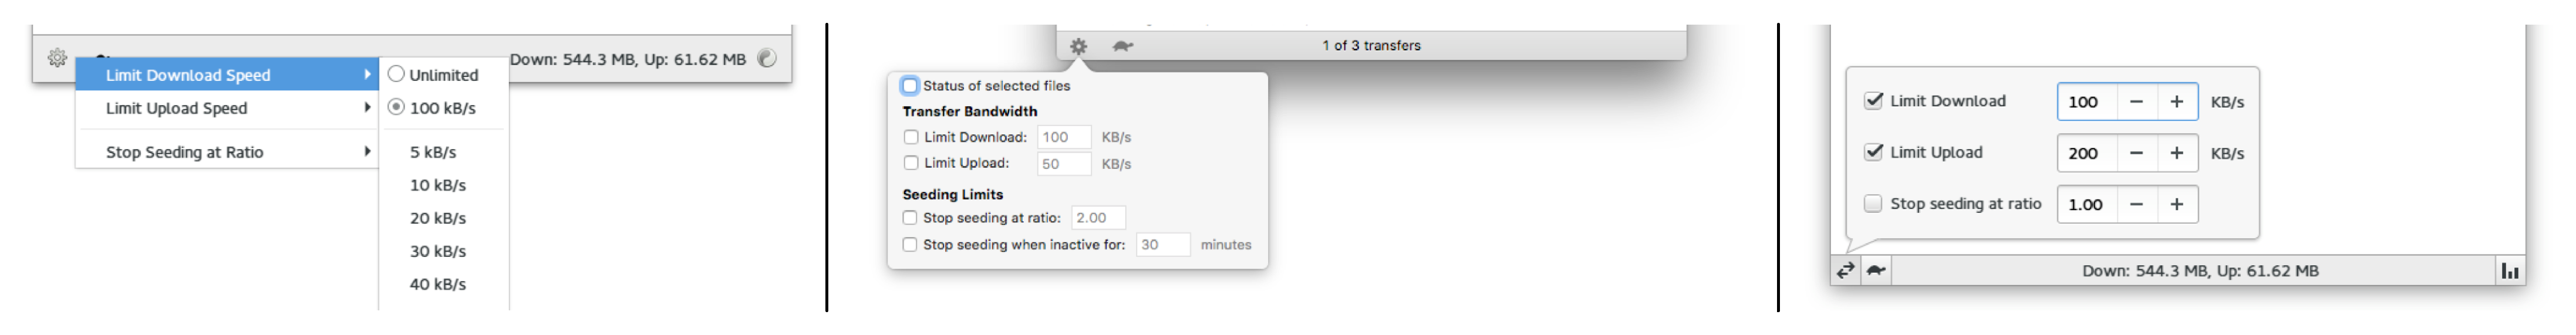
\includegraphics [width=\textwidth]{image/global-limits-transition.eps}
    \label{global-limits-transition}
    \fonte{Do Autor (2015)}
  \end{center}
\end{figure}

\subsection{Barra de Estado}

Inspirada na barra de estado do \textit{Gedit}, de altura compacta, e
utilizando-se das facilidades do GTK+ 3, todos os botões da barra de estado
foram implementados utilizando ícones simbólicos, de forma a se adaptarem a
temas claros e escuros (ilustrado na \autoref{status-bar}). Para implementar as
opções de visualização das estatísticas (último botão da esquerda para a
direita) foi utilizado um \textit{Popover}.

\begin{figure}[!ht]
  \begin{center}
    \caption{\textbf{Ícones simbólicos na barra de estado}}
    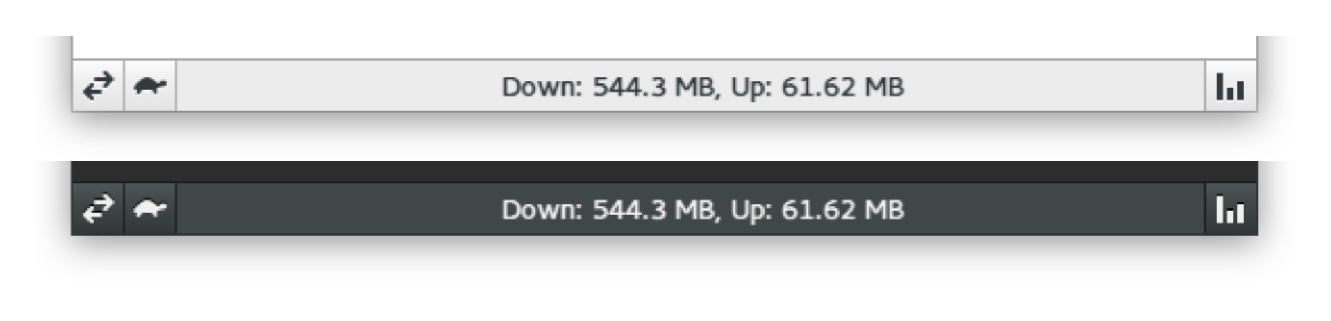
\includegraphics [width=\textwidth]{image/status-bar.eps}
    \label{status-bar}
    \fonte{Do Autor (2015)}
  \end{center}
\end{figure}


\chapter{CONCLUSÃO}

\bibliography{content/referencias}

\label{nropaginas}

\printindex

\end{document}
